% Generated numerical figure environments from main.tex.
\begin{figure}[t]
\centering
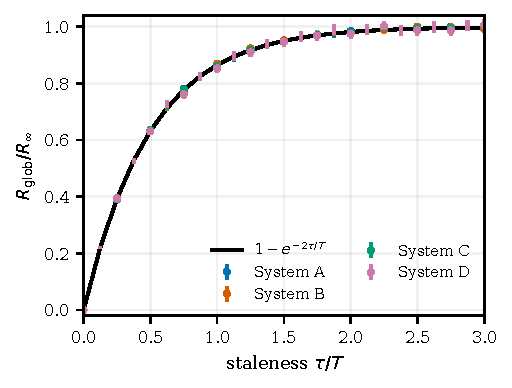
\includegraphics[width=0.82\linewidth]{numerics/figures/pdf/fig7_1_temporal_scaling.pdf}
\caption{Temporal scaling collapse from exact stationary OU pairs. Markers are
Monte Carlo estimates for four systems with different dimensions, spatial
covariances, objective matrices, and decision operators; bars are 95\%
confidence intervals. The solid curve is the exact law
$1-e^{-2\tau/T}$. Normalization by $R_\infty$ removes system-specific scale.}
\label{fig:temporal-scaling}
\end{figure}

\begin{figure}[t]
\centering
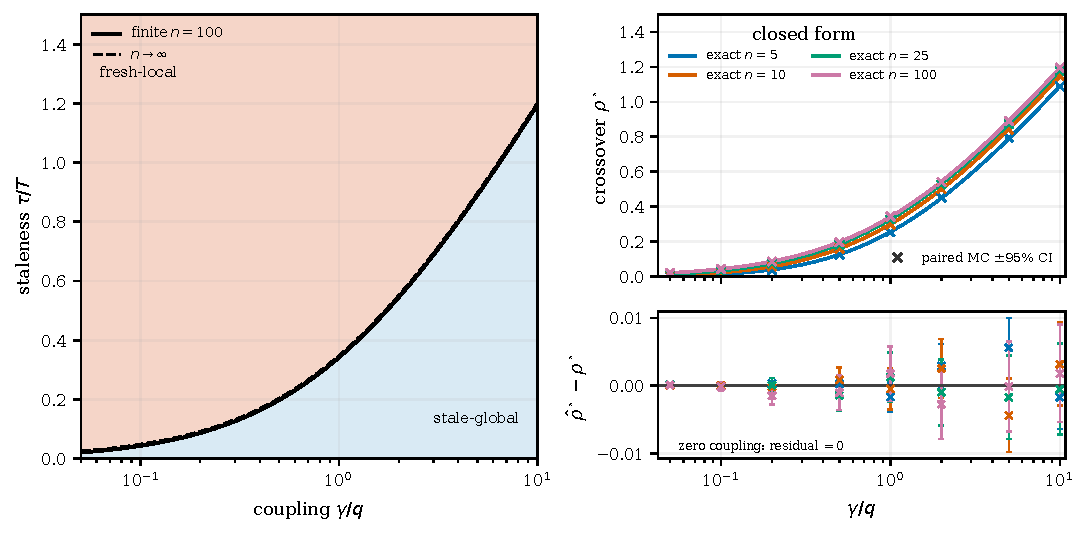
\includegraphics[width=0.98\linewidth]{numerics/figures/pdf/fig7_2_local_global_phase.pdf}
\caption{Fresh-local versus stale-global crossover. Left: the phase map uses the
exact finite-$n=100$ boundary (solid) and the large-$n$ limit (dashed),
Eqs.~\eqref{eq:aggregate_rho_star} and \eqref{eq:large_n_threshold}.
Upper right: exact theory curves and inferred Monte Carlo
boundaries (crosses) for four system sizes, with paired delta-method 95\%
intervals. Lower right: empirical minus theoretical boundary, on a scale that
reveals the sampling differences and their uncertainty.
The zero-coupling setting is evaluated at $\rho^\star=0$ but omitted from the
logarithmic positive-coupling axes.}
\label{fig:local-global-phase}
\end{figure}

\begin{figure}[t]
\centering
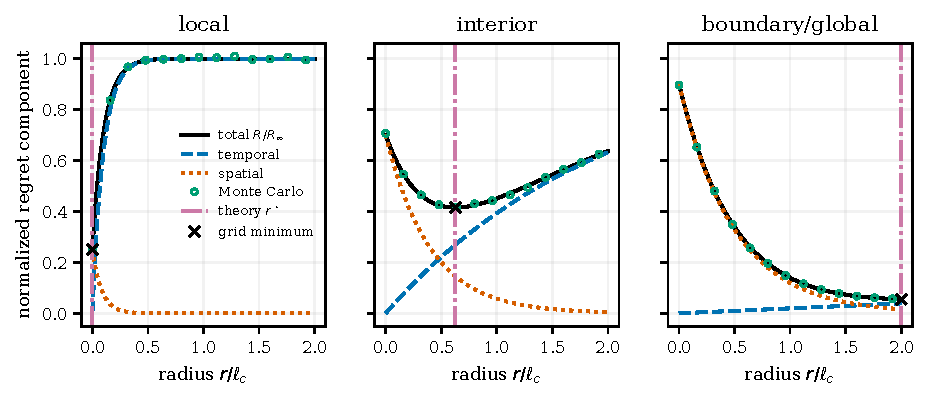
\includegraphics[width=\linewidth]{numerics/figures/pdf/fig7_3_radius_regret.pdf}
\caption{Emergence of local, interior, and maximum allowed radius optima under
$\eta_S(r)=\eta_0e^{-2r/\ell_c}$ and $\tau(r)=r/v$. Curves show total regret
and its temporal and residual-spatial terms from Eq.~\eqref{eq:R_decomposition};
open markers with 95\% intervals are independent scalar-innovation estimates.
Dash-dotted lines and crosses mark the analytical constrained and grid
minimizers. At the maximum allowed radius, positive omission remains:
$\eta_S(D)>0$.}
\label{fig:radius-regret}
\end{figure}

\begin{figure}[t]
\centering
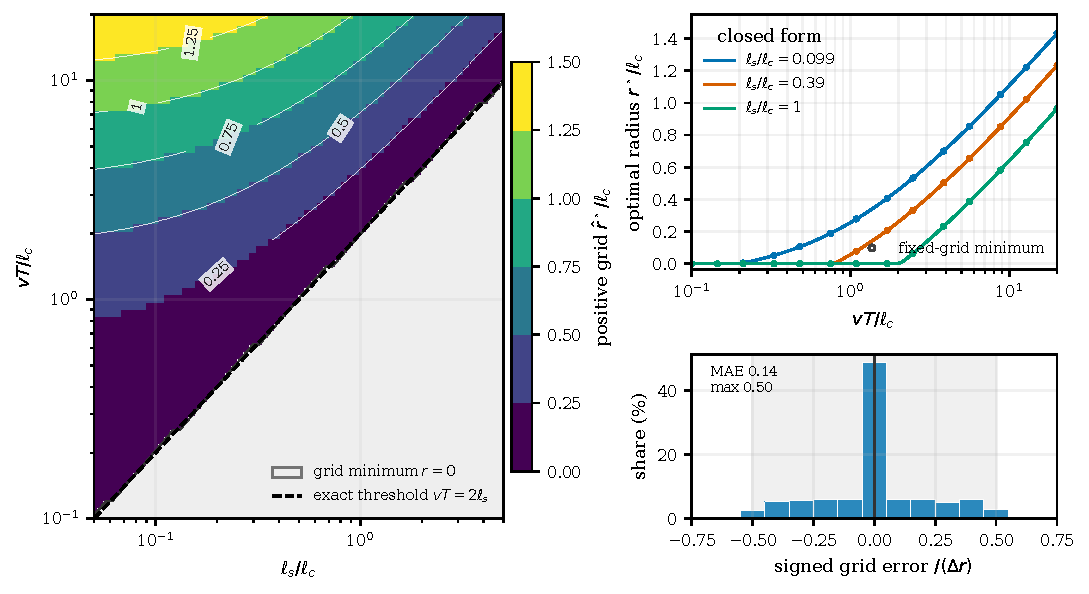
\includegraphics[width=0.98\linewidth]{numerics/figures/pdf/fig7_4_radius_phase.pdf}
\caption{Dimensionless optimal-radius law from direct scalar minimization. Left:
the numerical map, with the numerical zero-radius region shown in gray and the
dashed curve marking the theoretical transition $vT=2\ell_s$. Upper right:
selected $\ell_s/\ell_c$ slices comparing grid minimizers with the closed form
in Eq.~\eqref{eq:canonical_dimensionless_law}. Lower right: the histogram of
$(\hat r^\star-r^\star)/\Delta r$ over all 4,896 points; its zero spike
includes local-regime points and the remaining grid errors are of order a
half-step.}
\label{fig:radius-phase}
\end{figure}

\begin{figure}[t]
\centering
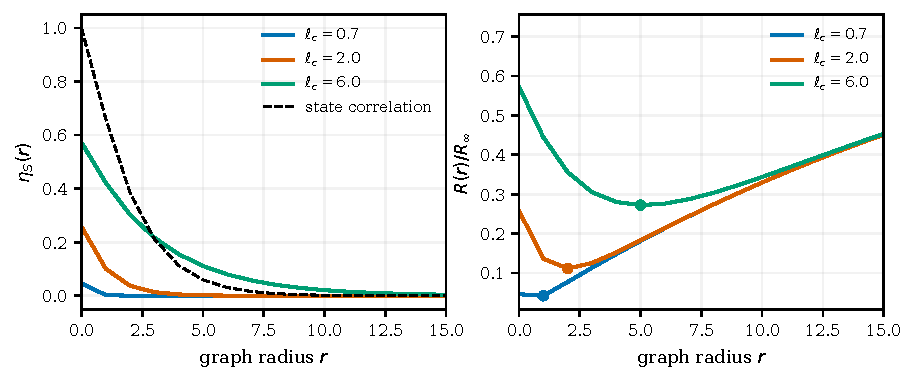
\includegraphics[width=0.94\linewidth]{numerics/figures/pdf/fig7_5_decision_relevance.pdf}
\caption{Decision relevance with the graph and state covariance held fixed.
The decision-weighted omission and normalized composed regret are shown for
three row-$\ell_2$-normalized operators with $Q=I$.  Raw state correlation is
shown in a separate context panel and is identical across operators; it is
not an omission estimate.  Each regret is normalized by its operator-specific
$R_\infty$, and the minimizing integer radius is marked.  Changing only the
decision-relevance range moves the optimum from 1 to 5 hops.}
\label{fig:decision-relevance}
\end{figure}

\begin{figure}[p]
\centering
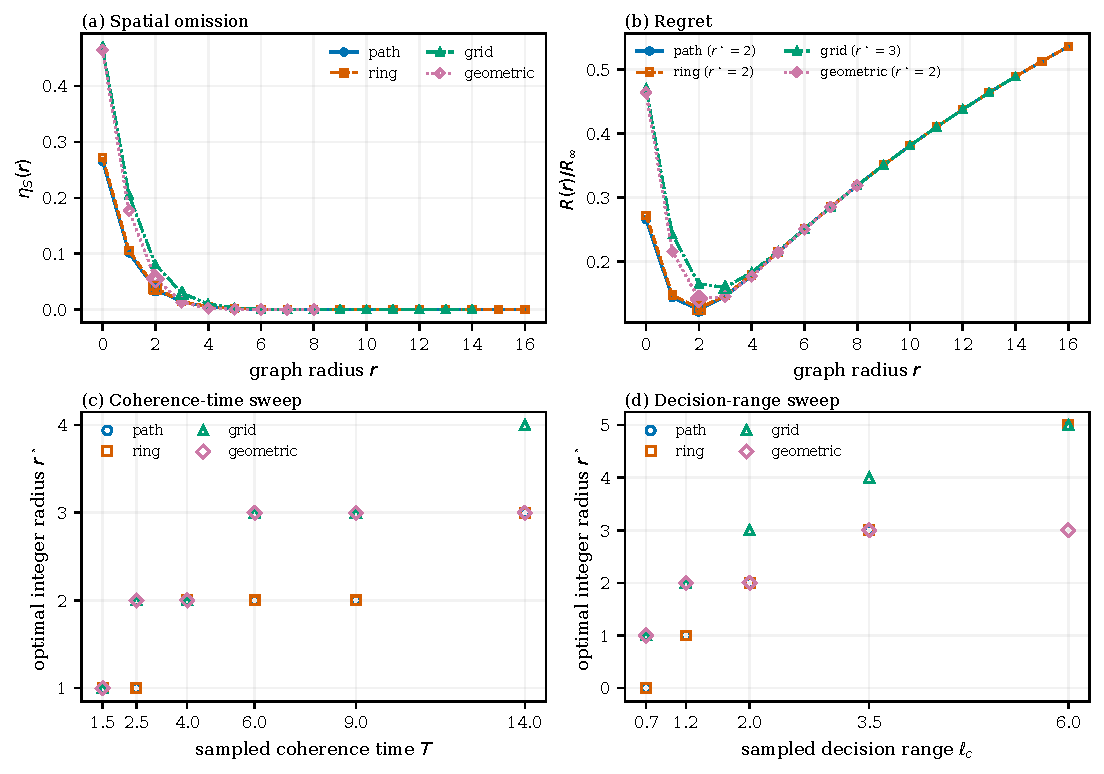
\includegraphics[width=\linewidth]{numerics/figures/pdf/fig7_6_general_graphs.pdf}
\caption{Finite noncanonical graphs. Top: $\eta_S(r)$ computed from exact
Gaussian conditional covariances and the resulting regret under one common
normalized setting; lines join integer-radius evaluations. Bottom: exact
integer optima at the sampled coherence times and decision ranges; no
transition locations between those settings are inferred. Distinct marker
shapes identify coincident graph results. The canonical line closed form is
not used.}
\label{fig:general-graphs}
\end{figure}
